\section{Zielsetzung}
\label{sec:Zielsetzung}
In diesem Versuch werden zwei gekoppelte Pendel untersucht. Ziel ist es, die Schwingungs- und Schwebungsdauern~$T$ und~$T_{\symup{S}}$, sowie die
Kopplungskonstante $\kappa$ zu bestimmen. Dafür werden gleichsinnige, gegensinnige und gekoppelte Schwingungen betrachtet.

\section{Theorie}
\label{sec:Theorie}
Wird ein Fadelpendel der Länge $l$ in dem Gravitationsfeld der Erde um einen kleinen Winkel $\varphi$ ausgelenkt, so ist die rücktreibende Kraft
proportional zur Auslenkung $x$ aus der Ruhelage. Hierbei handelt es sich somit um eine harmonische Schwingung die mit der Diffenentialgleichung für
den harmonischen Oszillator beschrieben werden kann. Die rücktreibende Kraft bewirkt ein Drehmoment $M=D_{\symup{P}}\varphi$, wobei $D_{\symup{P}}$
hierbei die Winkelrichtgröße des Pendels ist. Die Diffenentialgleichung der Bewegung des Pendels lautet dann:
\begin{align*}
    J\ddot{\varphi} + D_{\symup{P}}\varphi = 0
\end{align*}
Die Größe $J$ ist hier das Trägheitsmoment des Pendels.
Die Kreisfrequenz $\omega$ und die Schwingungsdauer $T$ folgen dann als
\begin{align}
    \omega &= \sqrt{\frac{g}{l}} \label{eq:Kreisfrequenz} \\
    T &= 2\symup{\pi}\sqrt{\frac{l}{g}}. \label{eq:Schwingungsdauer}
\end{align}

Werden nun zwei identische Pendel miteinander über eine Feder gekoppelt, lässt sich das System weiterhin in geschlossener Form mit zwei gekoppelten
Diffenentialgleichungen beschreiben. Hier wirken aufgrund der Kopplung die Drehmomente $M_1=D_{\symup{F}}(\varphi_2-\varphi_1)$ und~$M_2=-M_1$:
\begin{align*}
    J\ddot{\varphi_{1}} + D_{\symup{P}} \varphi_{1} &= D_{\symup{F}}(\varphi_2-\varphi_1) \\
    J\ddot{\varphi_{2}} + D_{\symup{P}} \varphi_{2} &= D_{\symup{F}}(\varphi_1-\varphi_2)
\end{align*}

Im Folgenden werden drei verschiedene Schwingungsarten, die durch jeweils andere Anfangsbedingungen gegeben sind, betrachtet. Die Winkel $\alpha_1$ 
und $\alpha_2$ sind hierbei die Auslenkungen aus der Ruhelage der Pendel zum Zeitpunkt $t=0$. Zu diesem Zeitpunkt befinden sich die Pedel in Ruhe, 
sodass darüber hinaus $\dot{\alpha_1}(t=0) = \dot{\alpha_2}(t=0) = 0$ gilt. \\


\underline{\textbf{1. Fall:}} \textbf{Gleichsinnige Schwingung} ($\alpha_1=\alpha_2$) \\
Werden die gekoppelten und identischen Pendel um denselben Winkel $\alpha_1=\alpha_2$ ausgelenkt, wird die Kopplungsfeder weder gestreckt, noch gestaucht.
Aus diesem Grund sind die Schwingungsfrequenz und -dauer dieselben wie die der einzelnen Pendel:
\begin{align}
    \omega_{+} &= \sqrt{\frac{g}{l}} \label{eq:w+} \\
    T_{+} &= 2\symup{\pi}\sqrt{\frac{l}{g}} \label{eq:T+}
\end{align} \\


\underline{\textbf{2. Fall:}} \textbf{Gegensinnige Schwingung} ($\alpha_1=-\alpha_2$) \\
In dem Fall, dass die beiden Pendel um denselben Winkel in unterschiedliche Richtungen, also $\alpha_1=-\alpha_2$, ausgelenkt werden, bewirkt die
Kopplung durch die Feder eine jeweils gleich große und entgegengesetzte Kraft auf die Pendel. Die Pendel schwingen symmetrisch zur Achse zwischen den 
Pendeln mit der Frequenz und Periodendauer von
\begin{align}
    \omega_{-} &= \sqrt{\frac{g+2K}{l}} \label{eq:w-} \\
    T_{-} &= 2\symup{\pi} \sqrt{\frac{l}{g+2K}}. \label{eq:T-}
\end{align}
Aufgrund der Kopplung ist nun auch die Federkonstante $K$ eine Abhängigkeit. \\


\underline{\textbf{3. Fall:}} \textbf{Gekoppelte Schwingung} ($\alpha_1=0$, $\alpha_2\neq 0$) \\
Wird nur ein Pendel ausgelenkt, während sich das andere in seiner Ruhelage befindet, wird die Energie des ausgelenkten Pendels über die
Feder übertragen. Zunächst beginnt das Pendel langsam zu schwingen, wobei die Auslenkung weiter zunimmt, bis das andere Pendel vollständig in Ruhe ist.
Diese Prozess wiederholt sich immer wieder und wird als \textit{Schwebung} bezeichnet. Die Schwebungsdauer $T_{S}$ ist der Zeitraum zwischen zwei Ruhelagen
eines Pendels:
\begin{align}
    \omega_{\symup{S}} &= \omega_{+} - \omega_{-} \label{eq:w_S} \\
    T_{\symup{S}} &= \frac{T_{+}\cdot T_{.}}{T_{+}-T_{-}} \label{eq:T_S} 
\end{align} 
Somit lässt sich die zu erwartende Schwbungsdauer aus den Schwingungsdauern der gleich- und gegensinnigen Schwingungen bestimmen. Um das Maß der Kopplung
der Pendel anzugeben, wird die Kopplungskonstante $\kappa$ eingeführt:
\begin{equation}
    \kappa = \frac{\omega_{-}^2-\omega_{+}^2}{\omega_{-}^2+\omega_{+}} = \frac{T_{+}^2-T_{-}^2}{T_{+}^2+T_{-}^2} \label{eq:Kopplungskonstante}
\end{equation}


\begin{figure}
    \begin{subfigure}{0.31\textwidth}
      \centering
      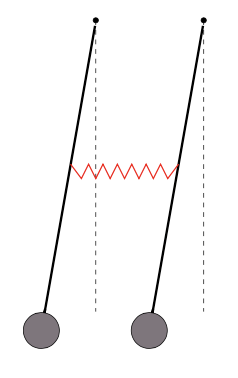
\includegraphics[height=5cm]{content/Bilder/Gleichsinnig.png}
      \caption{gleichsinnig}
      \label{fig:gleichsinnig}
    \end{subfigure}
    \hfill
    \begin{subfigure}{0.31\textwidth}
      \centering
      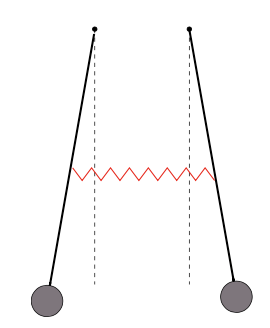
\includegraphics[height=5cm]{content/Bilder/Gegensinnig.png}
      \caption{gegensinnig}
      \label{fig:gegensinnig}
    \end{subfigure}
    \hfill
    \begin{subfigure}{0.31\textwidth}
      \centering
      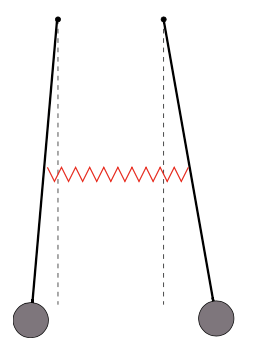
\includegraphics[height=5cm]{content/Bilder/Gekoppelt.png}
      \caption{gekoppelt}
      \label{fig:gekoppelt}
    \end{subfigure}
    \caption{Schematische Veranschaulichung der drei Schwingungsarten.\,\cite{v106}}
    \label{fig:Schema Schwingungsarten}
  \end{figure}